\subsection{Radiation Monitoring System}
\label{sec:RadiationDesign}

\subsubsection{MiniPIX Detector}
The MiniPIX detector, shown in Figure~\ref{fig:Minipix} is a silicon-based hybrid pixel detector built by ADVACAM~\cite{advacam} that utilizes technology developed by the MediPIX2 collaboration at CERN~\cite{medipix}. The sensor is composed of a pixellated silicon sensor integrated with a single TimePIX readout chip (256 x 256) pixels with a pitch of \SI{55}{\micro\meter}, the layers of the detector are shown in Figure~\ref{fig:MinipixLayers}. The sensor is \SI{500}{\micro\meter} thick and uses a USB 2.0 interface with a readout rate up to 30 frames per second. Each pixel can be programmed to work in one of three modes: Single particle counting, Time-over-Threshold (TOT), or Time-of-Arrival (TOA). This device offers a variety of applications including X-ray and neutron imaging as well as particle identification by characterizing each particle due to their charge, energy, and direction.

\begin{figure}[H]
  \begin{minipage}[c]{0.40\linewidth}
    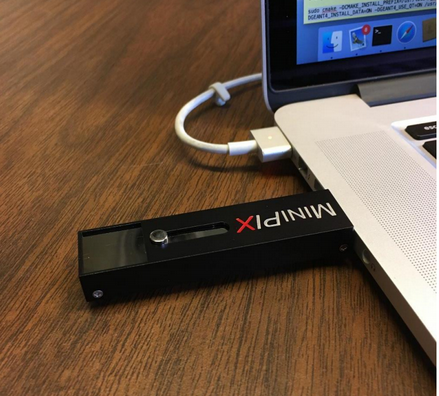
\includegraphics[width=\linewidth]{Figures/Minipix.png}
    \caption{Picture of a MiniPIX particle detector~\cite{advacam}.} %make sure to put figure names underneath the pictures
    \label{fig:Minipix}
  \end{minipage}
  \hfill
  \begin{minipage}[c]{0.45\linewidth}
    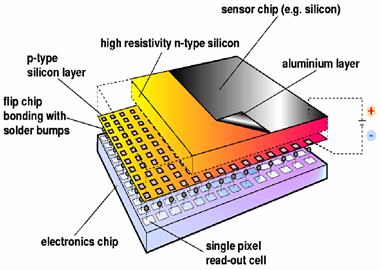
\includegraphics[width=\linewidth]{Figures/MinipixLayers.png}
    \caption{Hybrid pixel detector silicon sensor~\cite{silicon_sensor}.} %make sure to put figure names underneath the pictures
    \label{fig:MinipixLayers}
  \end{minipage}
\end{figure}

The MiniPIX registers ionized particles when the active material in the detector is transformed into a charge (the excitement of electron-hole pairs in the semiconductor). When these charges are collected, the Si bulk is then depleted by an applied bias voltage, which occurs when the electronics reads-out electron-hole pairs. If these pairs are above the threshold when collected by the pixel electronics, the count increases. The projection of the deposited charge is measured and the total energy deposited can be determined from the back-plane pulse amplitude. 

When a particle is incident on the sensor, a particle track is produced along the path length through the sensor area. The path of a single particle through the sensor is called the particle track.  Each particle track may be identified as a ``cluster'' or continuous area of neighboring pixels in a given frame. Each individual cluster can be differentiated through statistical analysis to describe the shape and energy deposition, allowing us to distinguish between different types of radiation by organizing each cluster into aspecific morphological category. 
%The feature parameters of this detector provides detailed information about total energy deposited by particles, and if only one particle is traced in the detector this tells us that slow heavy particles ionize more than fast moving ones. 

\begin{figure}[h]
  \begin{minipage}[c]{0.49\linewidth}
    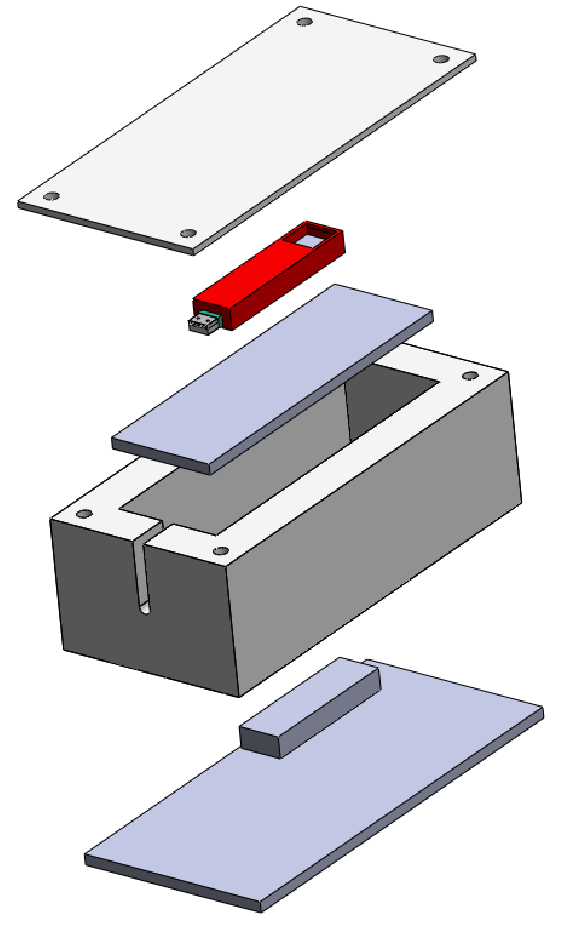
\includegraphics[scale=1, width=.5\textwidth]{Figures/MinipixCaseAssembly.pdf}
    \caption{3D rendering of the MiniPIX case and heat sink assembly.}
    \label{fig:CaseAssembly}
  \end{minipage}
  \hfill
  \begin{minipage}[c]{0.49\linewidth}
    \centering
    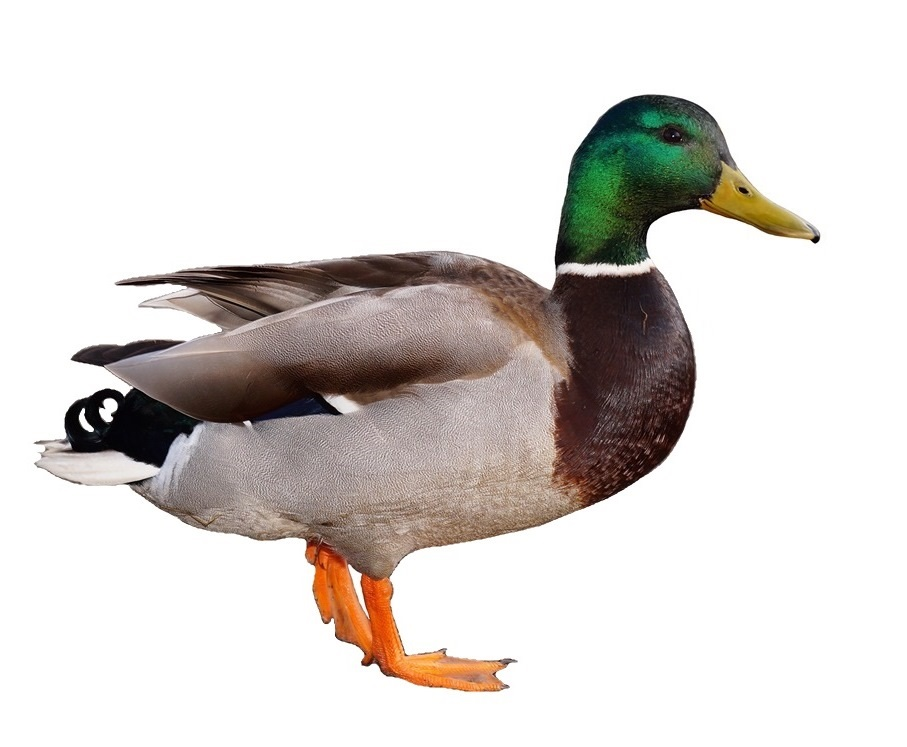
\includegraphics[scale=1, width=.5\textwidth]{Figures/duck.jpg}
    \caption{Picture of the MiniPIX mounted in the case and heat sink assembly on SORA 1.0.}
    \label{fig:CaseAssembly2}
  \end{minipage}
\end{figure}

The primary purpose of the MiniPIX is to detect four specific types of radiation: alpha $(\alpha)$, electron $({e^-})$, gamma $({\gamma})$, and muon $({\mu})$. By comparing the results of the flight to results obtained from simulations, an estimate regarding the percent composition of the detector hits can be made.

The MiniPIX case and heat sink assembly shown in Figure~\ref{fig:CaseAssembly} is designed to protect the device from any moisture in the atmosphere. The case and lid will be 3D printed using ABS plastic and the heat sink will be composed of two large sheets and a small block of aluminum metal which will all be mounted to the roof of the payload. Thermal paste will be applied at every contact point between the device and each of the aluminum pieces to allow for optimal thermal conduction and radiation of heat away from the MiniPIX. A picture of the MiniPIX device inside the case and heat sink assembly used on SORA 1.0 is shown in Figure~\ref{fig:CaseAssembly2}. Considering the success of that setup, we will mimic a similar configuration on SORA 2.0.

\subsubsection{Calibration}   
The appropriate calibration of the MiniPIX detector will be applied at The University of Houston by Dr.~Stuart P.~George, a collaborator within the MediPIX Collaboration. The source calibration will be applied using the \SI{60}{\keV} {\ce{^241Am} decay line, \ce{Sn} Fluorescence and \ce{^55Fe} gamma rays. The TimePIX hybrid pixel detector consists of \num{65536} silicon p-n diodes, with each containing its own individual processing circuit. The response of each pixel can never be identical, thus a calibration must be performed for each individual pixel. Dr.~George will calibrate the pixel energy threshold from DAC counts to energy~\cite{stuartthesis}. The threshold will be set at \SI{4}{\keV}, just above the noise level of the detector. The set threshold energy of the TimePIX chip determines what energies of particles are allowed to be measured by the detector. Energy measurements in the detector are accounted by measuring the charge collected in each individual pixel. The sensor's bias voltage will be \SI{200}{\volt} to ensure that the sensor was completely depleted. 
  
\subsubsection{Collection Parameters}
% Put the settings for the minipix shutter time, bias voltage etc. here
The device will be configured via the device Python API wrapper provided by ADVACAM. Acquisition parameters will be determined through testing. This time must be chosen as a balance between too many individual frames with little to no data, which would take up a lot of storage space, and individual frames that are so crowded with interactions that they are unreadable due to a large number of crossed tracks. Upon completing an acquisition, the device enters a manufacturer-set dormant state for approximately two seconds, which will be utilized as cool-down period and to record the internal temperature of the device into a .csv file.

\subsubsection{Data Format}
The data format for each frame of data is a plain text array with each value corresponding to the value at the corresponding pixel index in the detector. Upon the capture of a new frame the plain text array will be appended to the acquisition file stored on the SD card of the RP\num{3} on our payload. In a separate file various metadata will be stored for each frame including the detector threshold, acquisition time, acquisition mode etc. The plaintext array format means that each frame of data utilized approximately \SI{132}{\kilo\byte} of memory. In SORA \num{1.0}, a frame was saved roughly every six seconds, over the course of the roughly fourteen hour flight we had a total acquisition size of approximately \SI{1.1}{\giga\byte}. While this was a rather small total collection size, we could have further reduced our memory footprint by only storing pixel indices with non-zero time over threshold values i.e.\ storing data in a sparse matrix format. This is a route we will look into for SORA \num{2.0}.
